% beamer 16:9
\documentclass[aspectratio=169, 9pt, xcolor=dvipsnames]{beamer}
\usecolortheme[named=NavyBlue]{structure}
\beamertemplatenavigationsymbolsempty
\setbeamertemplate{footline}[frame number]
\usefonttheme{serif}
\setbeamertemplate{caption}[numbered]
\setbeamerfont*{itemize/enumerate subbody}{parent=itemize/enumerate body}
% math package
\usepackage{amsmath, amsthm, amssymb, booktabs, multirow, hyperref, pgffor, tabularx, makecell}
\usepackage{kotex}
\usepackage[backend=bibtex,style=authoryear]{biblatex}
\newcolumntype{C}{ >{\centering\arraybackslash} m{1cm} }
\newcolumntype{D}{ >{\centering\arraybackslash} m{3.5cm} }

\title{시나리오 별 서울, 경기 지역 코로나 확진자 수 및 위중증 환자 수 예측}
\author{이윤정 \inst{1} \and 석정주 \inst{2} \and 이지현 \inst{2}}
\institute{\inst{1} 연세대학교 수학계산학부 (계산과학공학과) \and \inst{2} 연세대학교 수학계산학부 (수학과)}
\date{\today}

\addbibresource{210909_ref.bib}

\begin{document}
	
	\begin{frame}\frametitle{}
	    \maketitle
	\end{frame}

	\begin{frame}\frametitle{데이터}
	    \begin{enumerate}
	    	\item 서울, 경기 일일 발생 확진자 수
	    	\item 백신
	    	\begin{itemize}
	    		\item 연령별 백신 접종량
	    		\item $\alpha$ 변이 $\rightarrow$ $\delta$ 변이에 따른 백신 효과
	    	\end{itemize}
	    	\item 사용 중인 위중증 병상 수
	   	\end{enumerate}
	\end{frame}

	\begin{frame}\frametitle{데이터}
	    \textbf{일일 백신 접종량 (전 연령)}
	    \begin{figure}
	    	\centering
	    	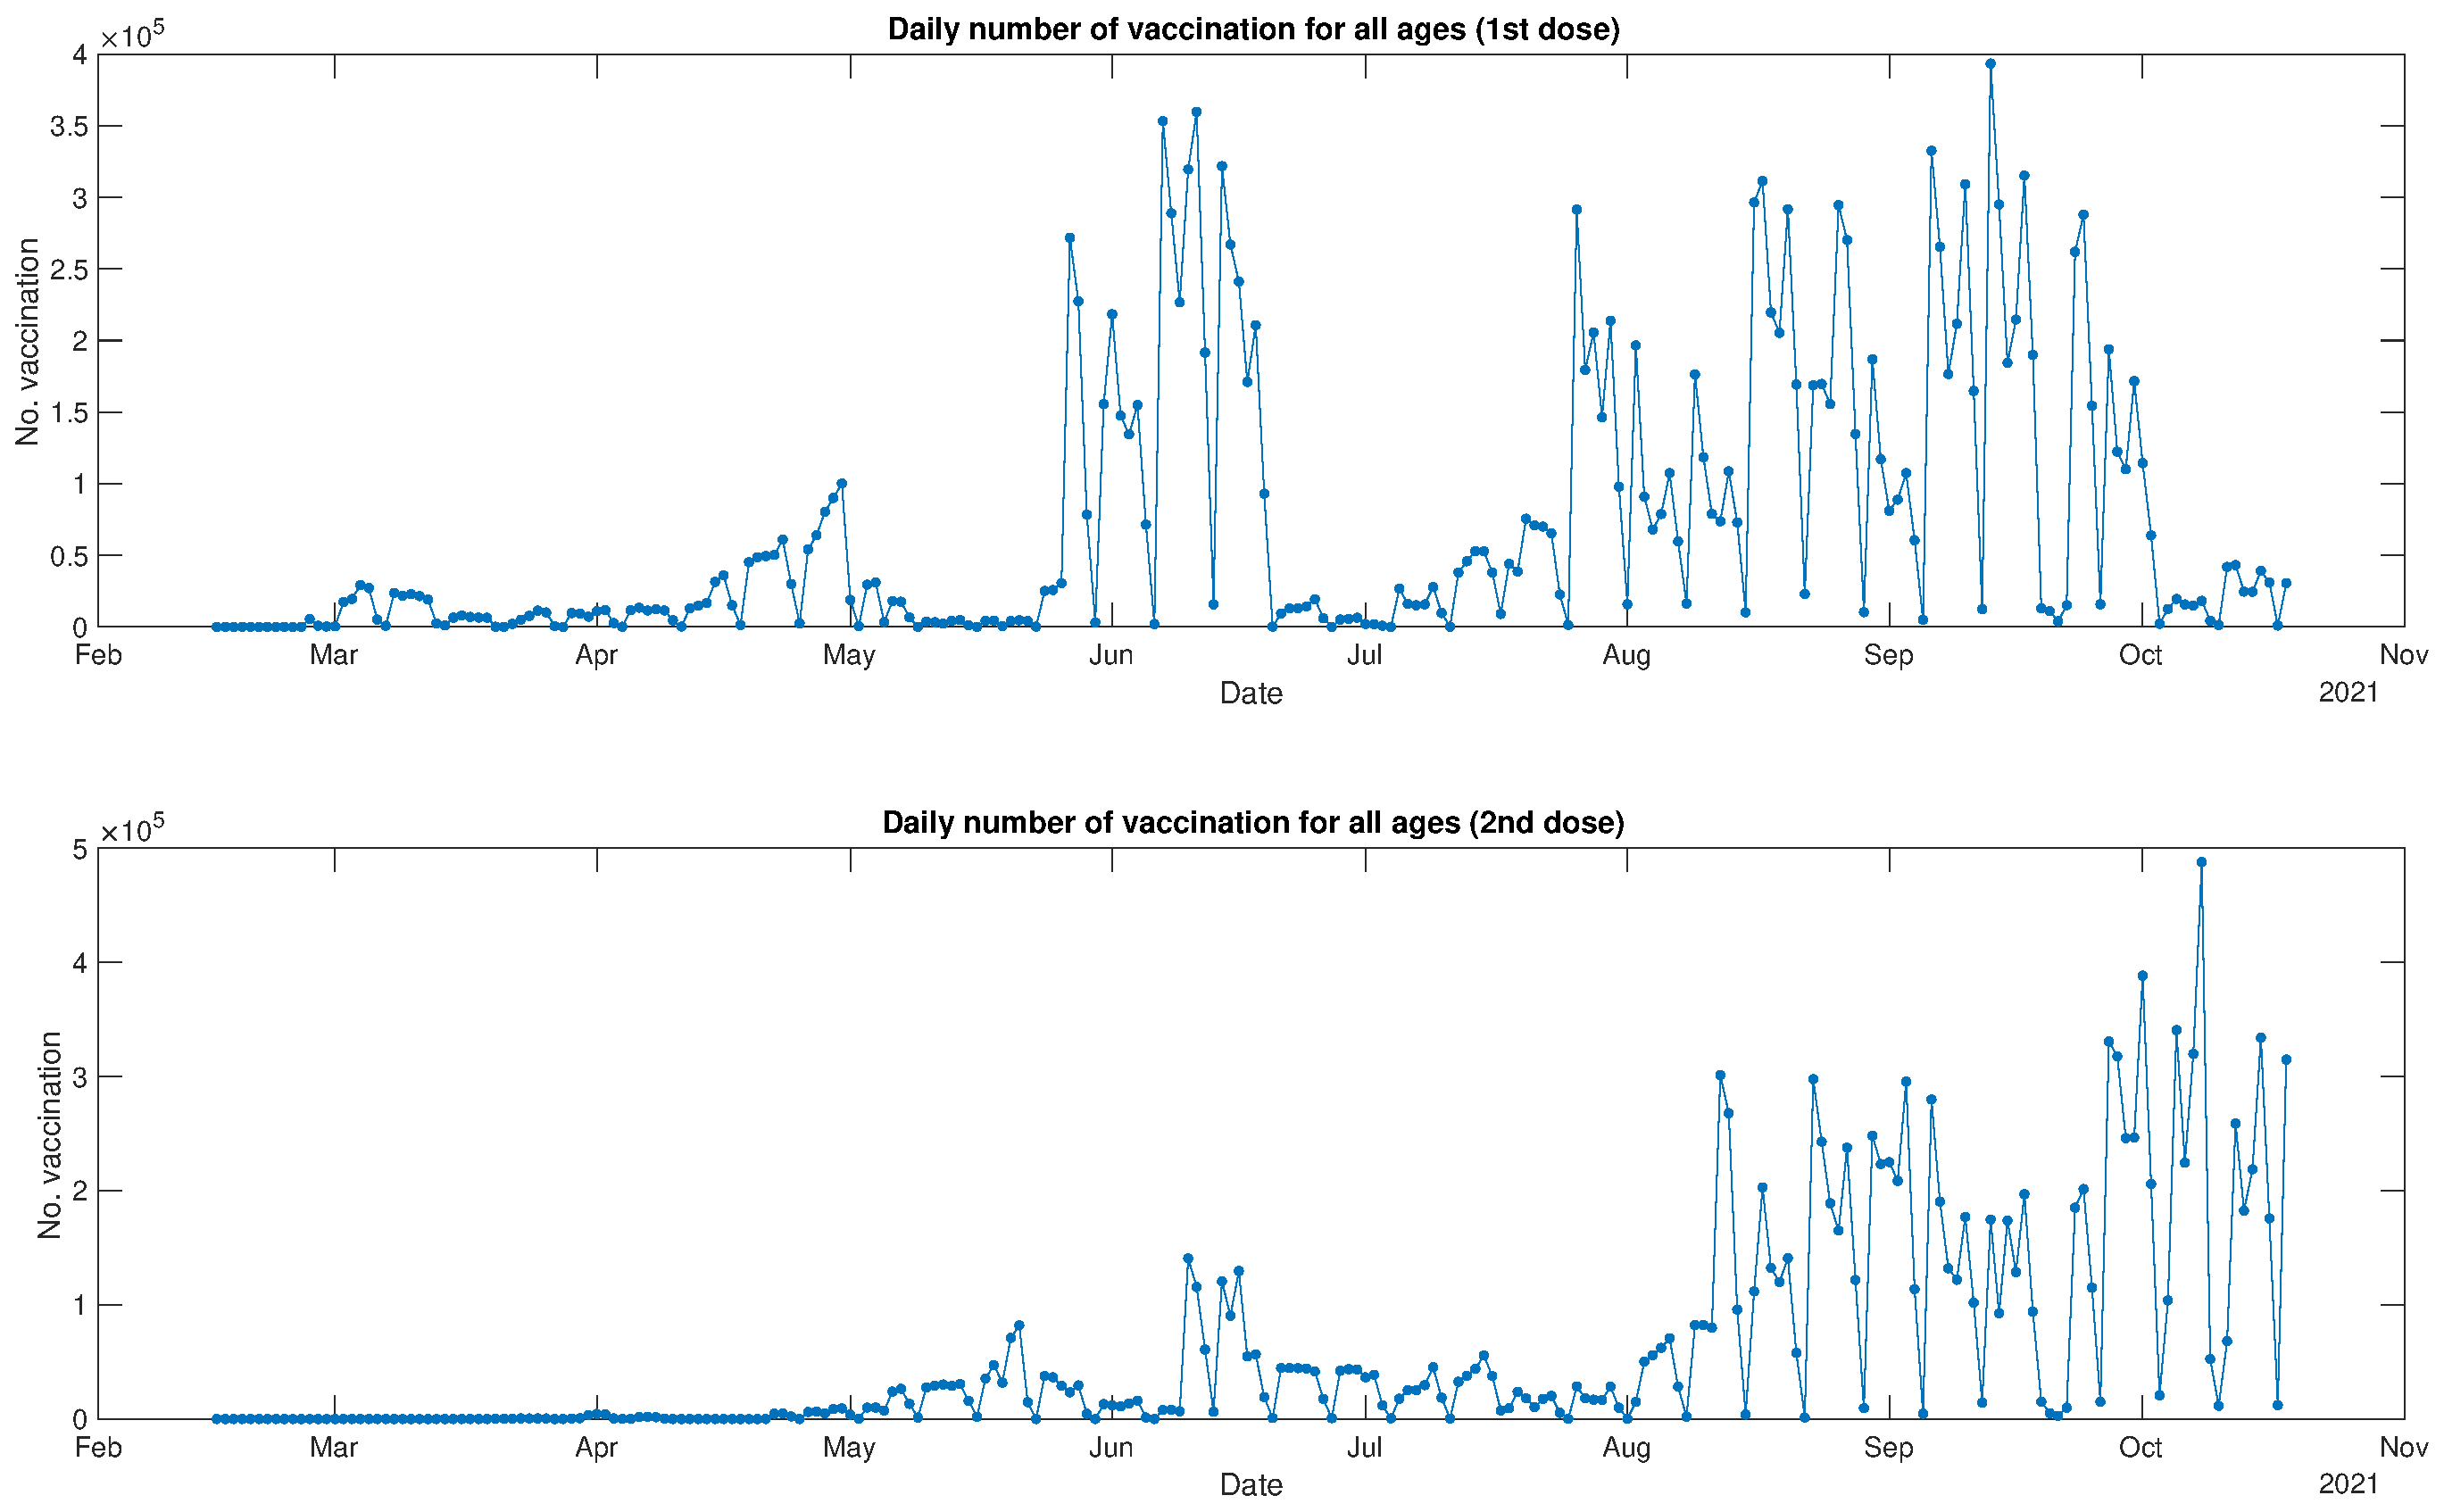
\includegraphics[width=10cm]{../results/data/vaccine_number.eps}
	    	\caption{2021/02/15-2021/10/21의 1차, 2차 백신 접종량.}
	    \end{figure}
	\end{frame}

	\begin{frame}\frametitle{데이터}
	    \textbf{연령별 일일 1차 백신 접종량}
	    \begin{itemize}
	    	\item 연령별 백신 접종량은 전국의 연령별 백신 접종 비율로부터 추산
	    	\item 연령별 백신 비율은 질병관리청의 보도자료를 이용
	    \end{itemize}
	    \begin{figure}
	    	\centering
	    	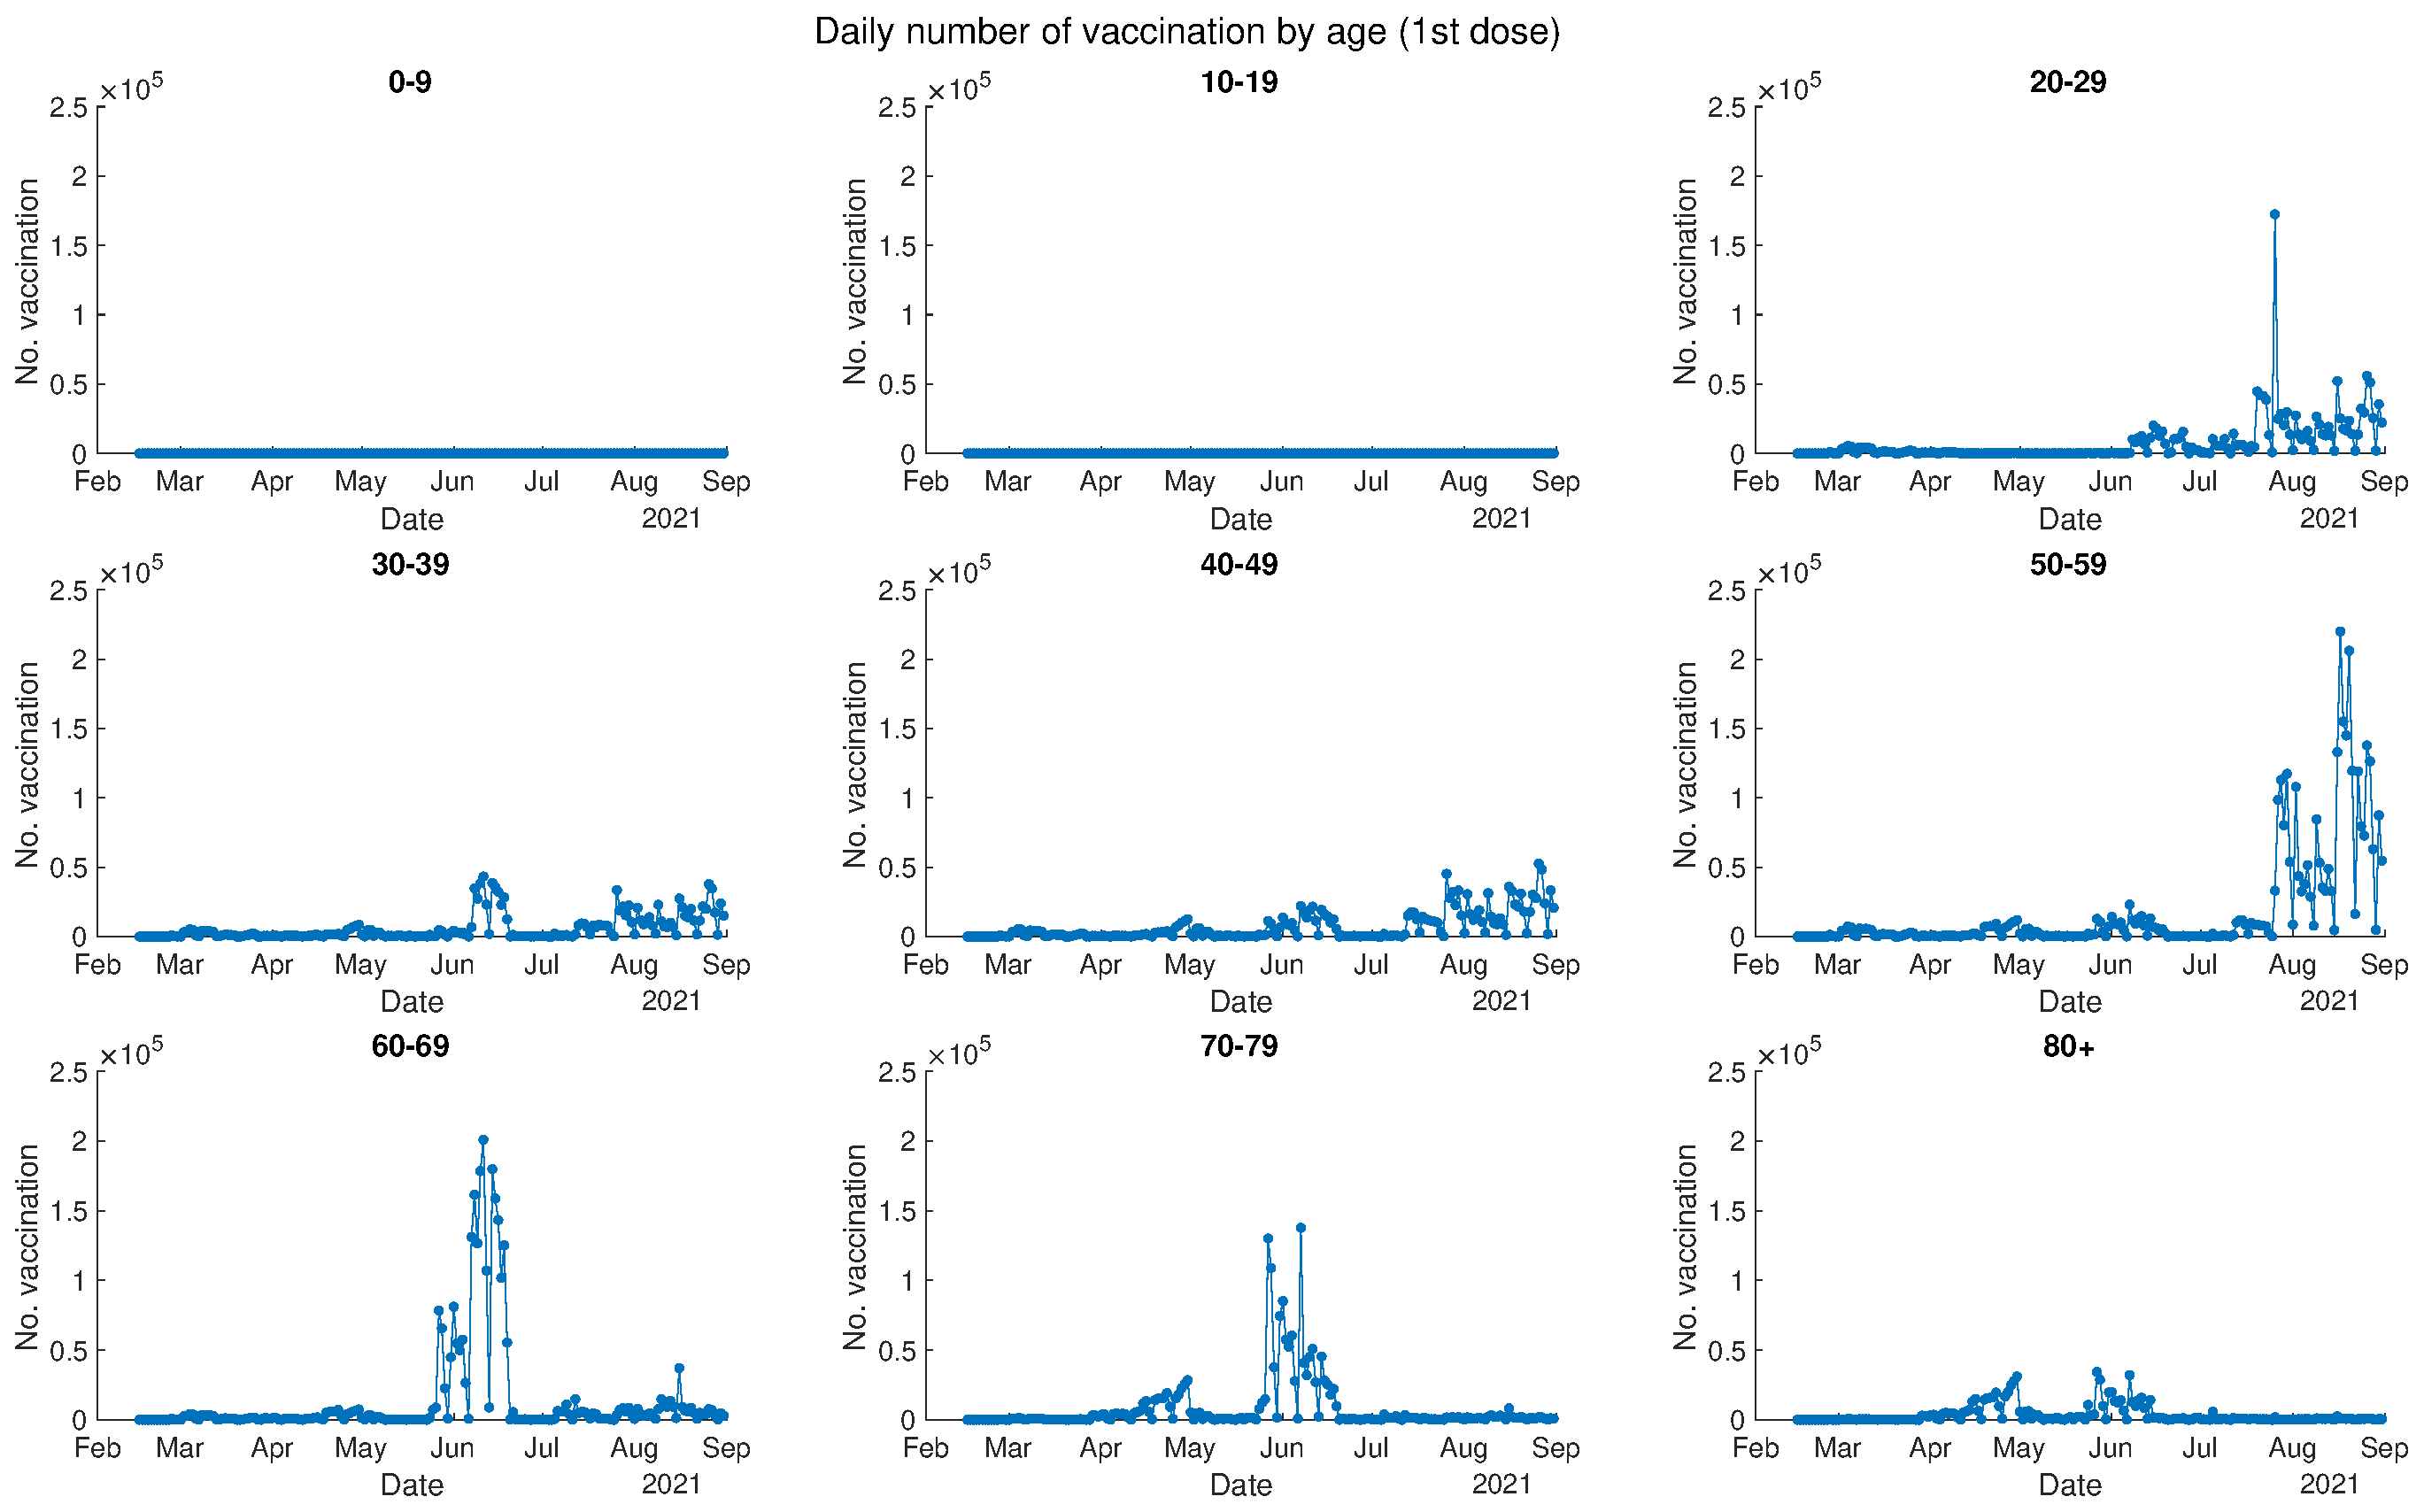
\includegraphics[width=8cm]{../results/data/vaccine_number_by_age_1st.eps}
	    	\caption{2021/02/15-2021/10/18의 연령별 일일 1차 백신 접종량.}
	    \end{figure}
	\end{frame}

	\begin{frame}\frametitle{데이터}
	    \textbf{연령별 일일 2차 백신 접종량}
	    \begin{itemize}
	    	\item 연령별 백신 접종량은 전국의 연령별 백신 접종 비율로부터 추산
	    	\item 연령별 백신 비율은 질병관리청의 보도자료를 이용
	    \end{itemize}
	    \begin{figure}
	    	\centering
	    	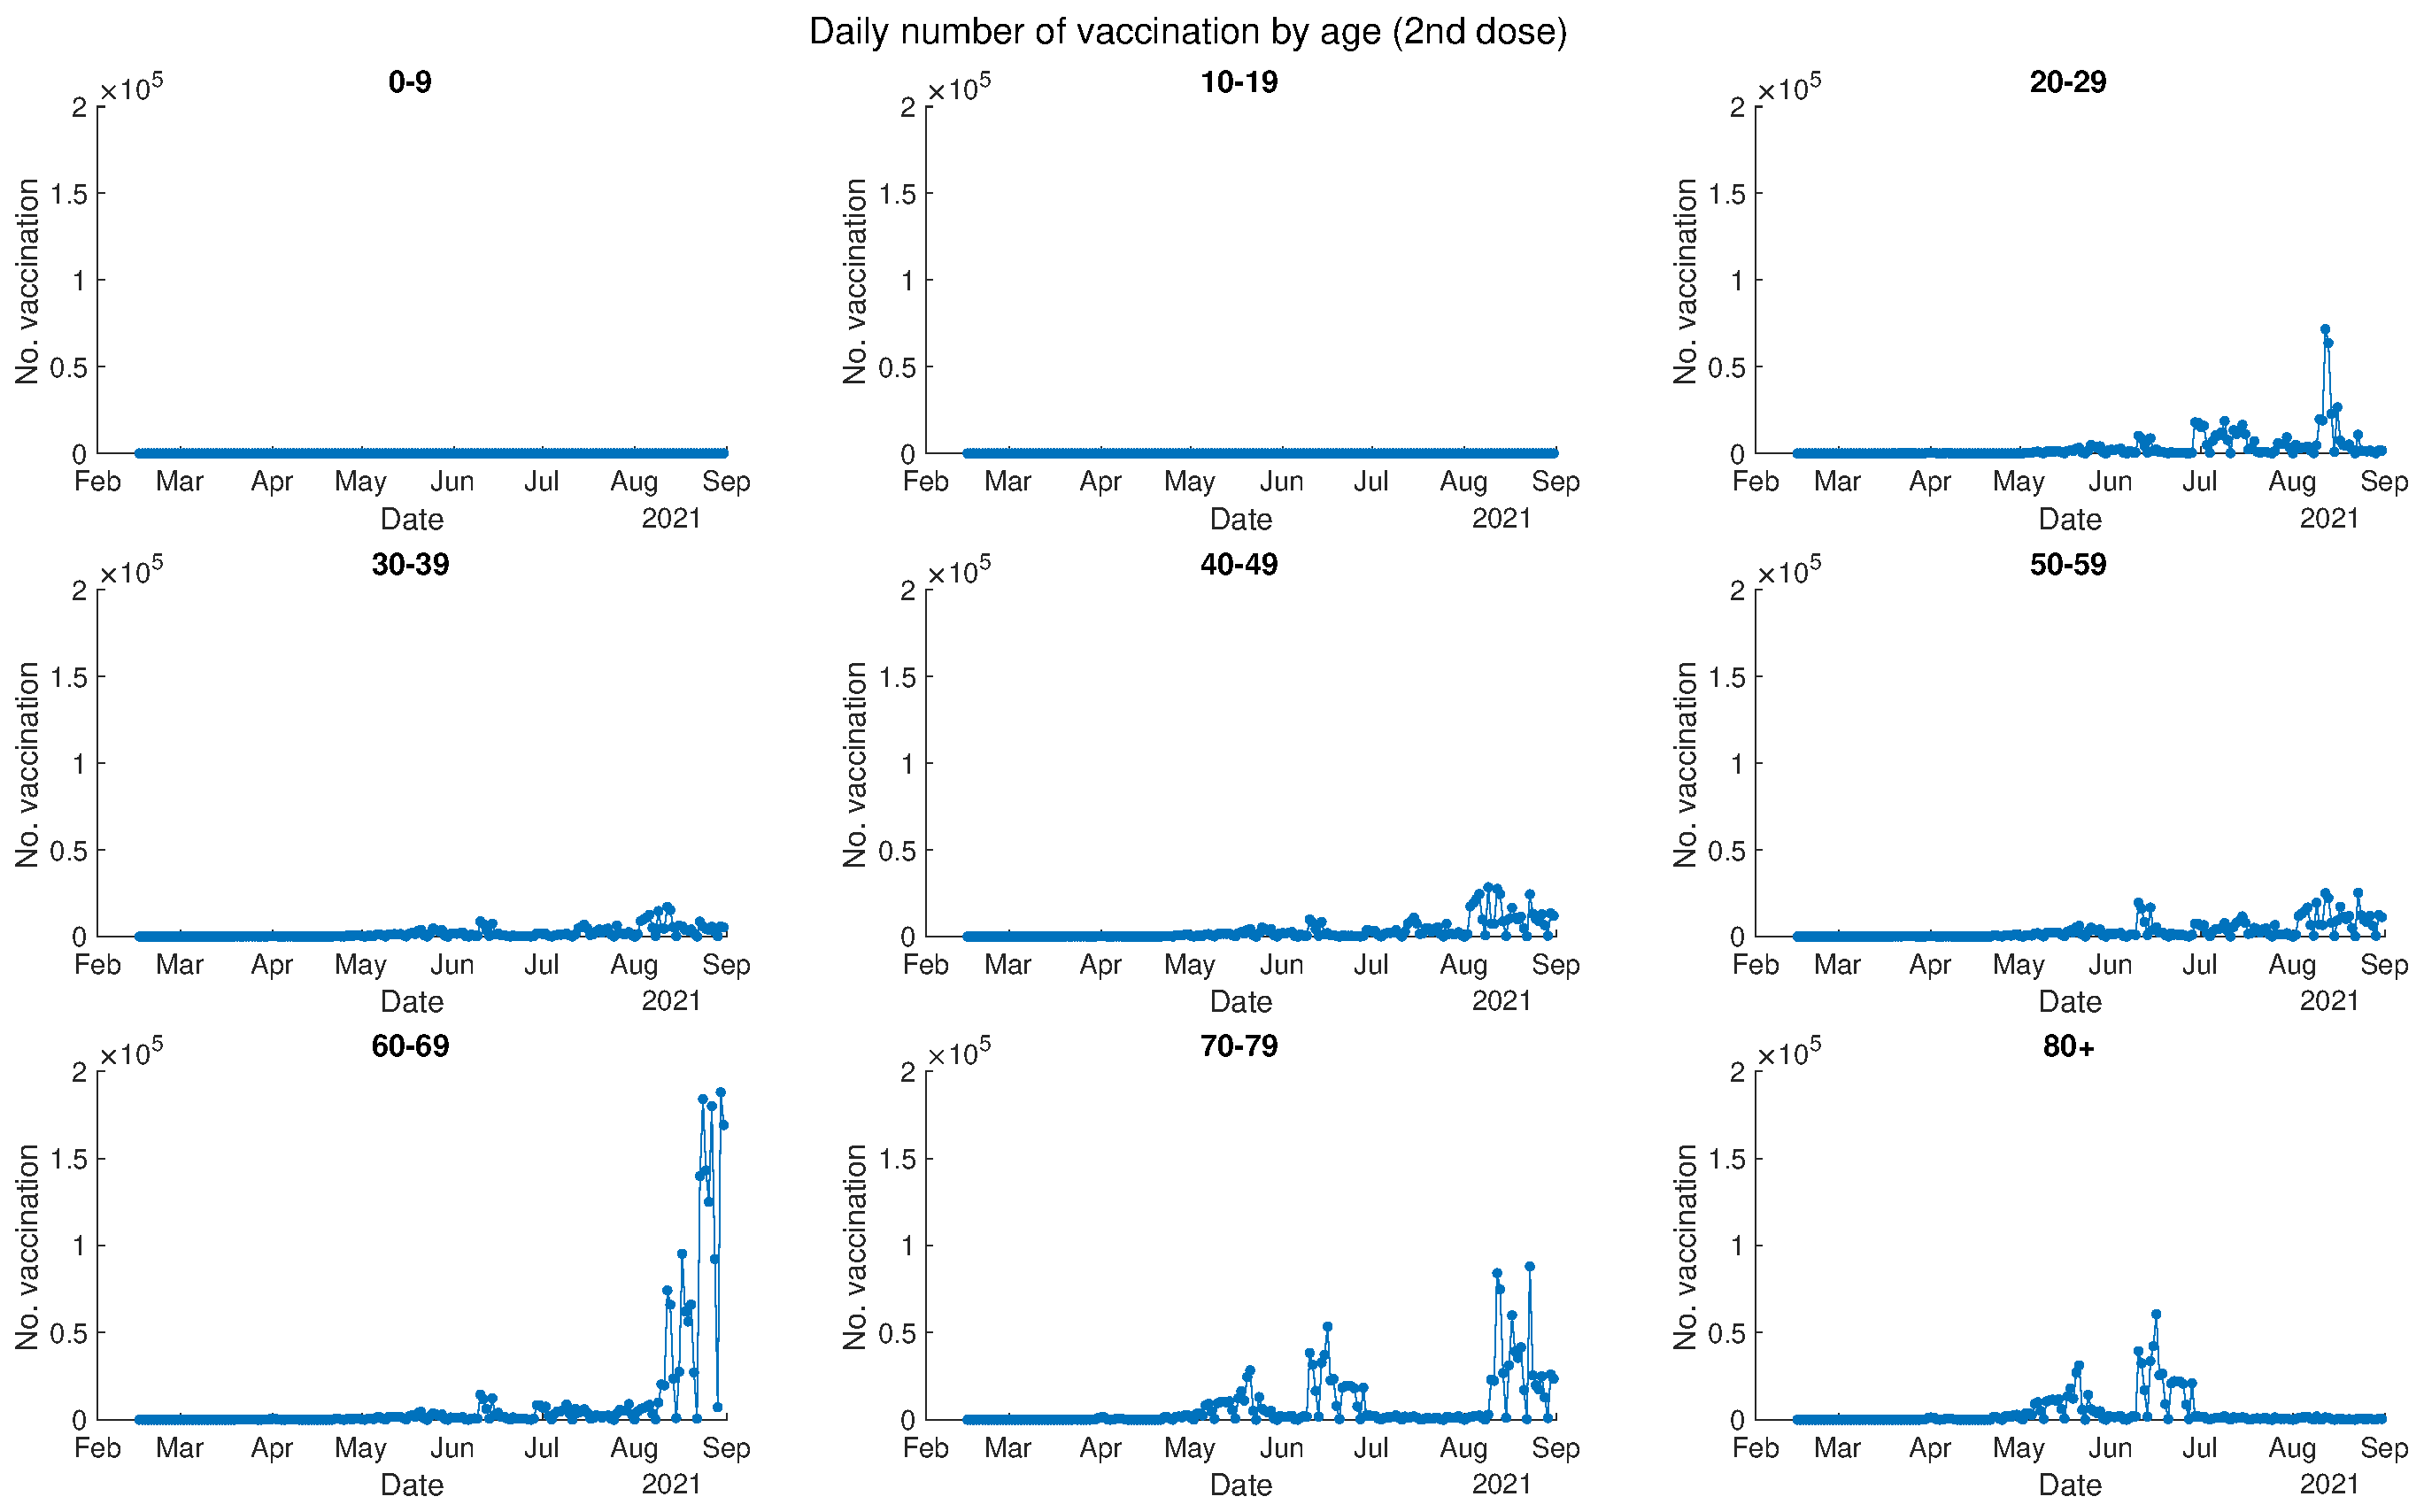
\includegraphics[width=8cm]{../results/data/vaccine_number_by_age_2nd.eps}
	    	\caption{2021/02/15-2021/10/18의 연령별 일일 2차 백신 접종량.}
	    \end{figure}
	\end{frame}

	\begin{frame}\frametitle{데이터}
	    \textbf{백신 효과}
		\begin{itemize}
			\item $\alpha$ 변이와 $\delta$ 변이에 대한 백신 효과는 서로 다름.\footnotemark[1]
		\end{itemize}
		\begin{table}
			\begin{tabular}{c|crr}
				\toprule
				& \textbf{Dose} & \textbf{Astrazeneca} & \textbf{Pfizer} \\
				\midrule
				\multirow{2}{*}{$\mathbf{\alpha}$ variant} & \textbf{1st dose} & 48.7\% & 47.5\% \\
				& \textbf{2nd dose} & 74.5\% & 93.7\% \\
				\midrule
				\multirow{2}{*}{$\mathbf{\delta}$ variant} & \textbf{1st dose} & 30.0\% & 35.6\% \\
				& \textbf{2nd dose} & 67\% & 88\% \\
				\bottomrule
			\end{tabular}
			\caption{백신 종류, 변이 바이러스 및 백신 차수에 따른 백신 효과.}
		\end{table}
		\footnotetext[1]{\fullcite{bernal2021effectiveness}}
	\end{frame}

		\begin{frame}\frametitle{데이터}
	    \textbf{백신 효과} \\
		\begin{itemize}
			\item $\delta$ 변이의 비율을 보도자료로부터 추정하고 weighted sum을 이용하여 백신 효과를 추정.
		\end{itemize}
	    \begin{minipage}{0.3\textwidth}
	    	\begin{table}
	    		\resizebox{\textwidth}{!}{
	    		\begin{tabular}{lr}
	    			\toprule
	    			\textbf{Date} & \textbf{$\delta$ proportion (\%)} \\
	    			\midrule
	    			6월 1주차 & 2.4 \\
	    			6월 2주차 & 1.4 \\
	    			6월 3주차 & 2.5 \\
	    			6월 4주차 & 3.3 \\
	    			6월 5주차 & 9.9 \\
	    			7월 1주차 & 23.3 \\
	    			7월 2주차 & 33.9 \\
	    			7월 3주차 & 48.0 \\
	    			7월 4주차 & 61.5 \\
	    			8월 1주차 & 73.1 \\
	    			8월 2주차 & 85.3 \\
	    			8월 3주차 & 89.6 \\
	    			8월 4주차 & 94.3 \\
	    			9월 1주차 & 97.0 \\
	    			\bottomrule
	    		\end{tabular}
	    		}
	    		\caption{질병관리청에서 보도된 검출된 델타 변이 비율}
	    	\end{table}
	    \end{minipage}
	    \hfill
	    \begin{minipage}{0.6\textwidth}
	    	\begin{figure}
	    		\centering
	    		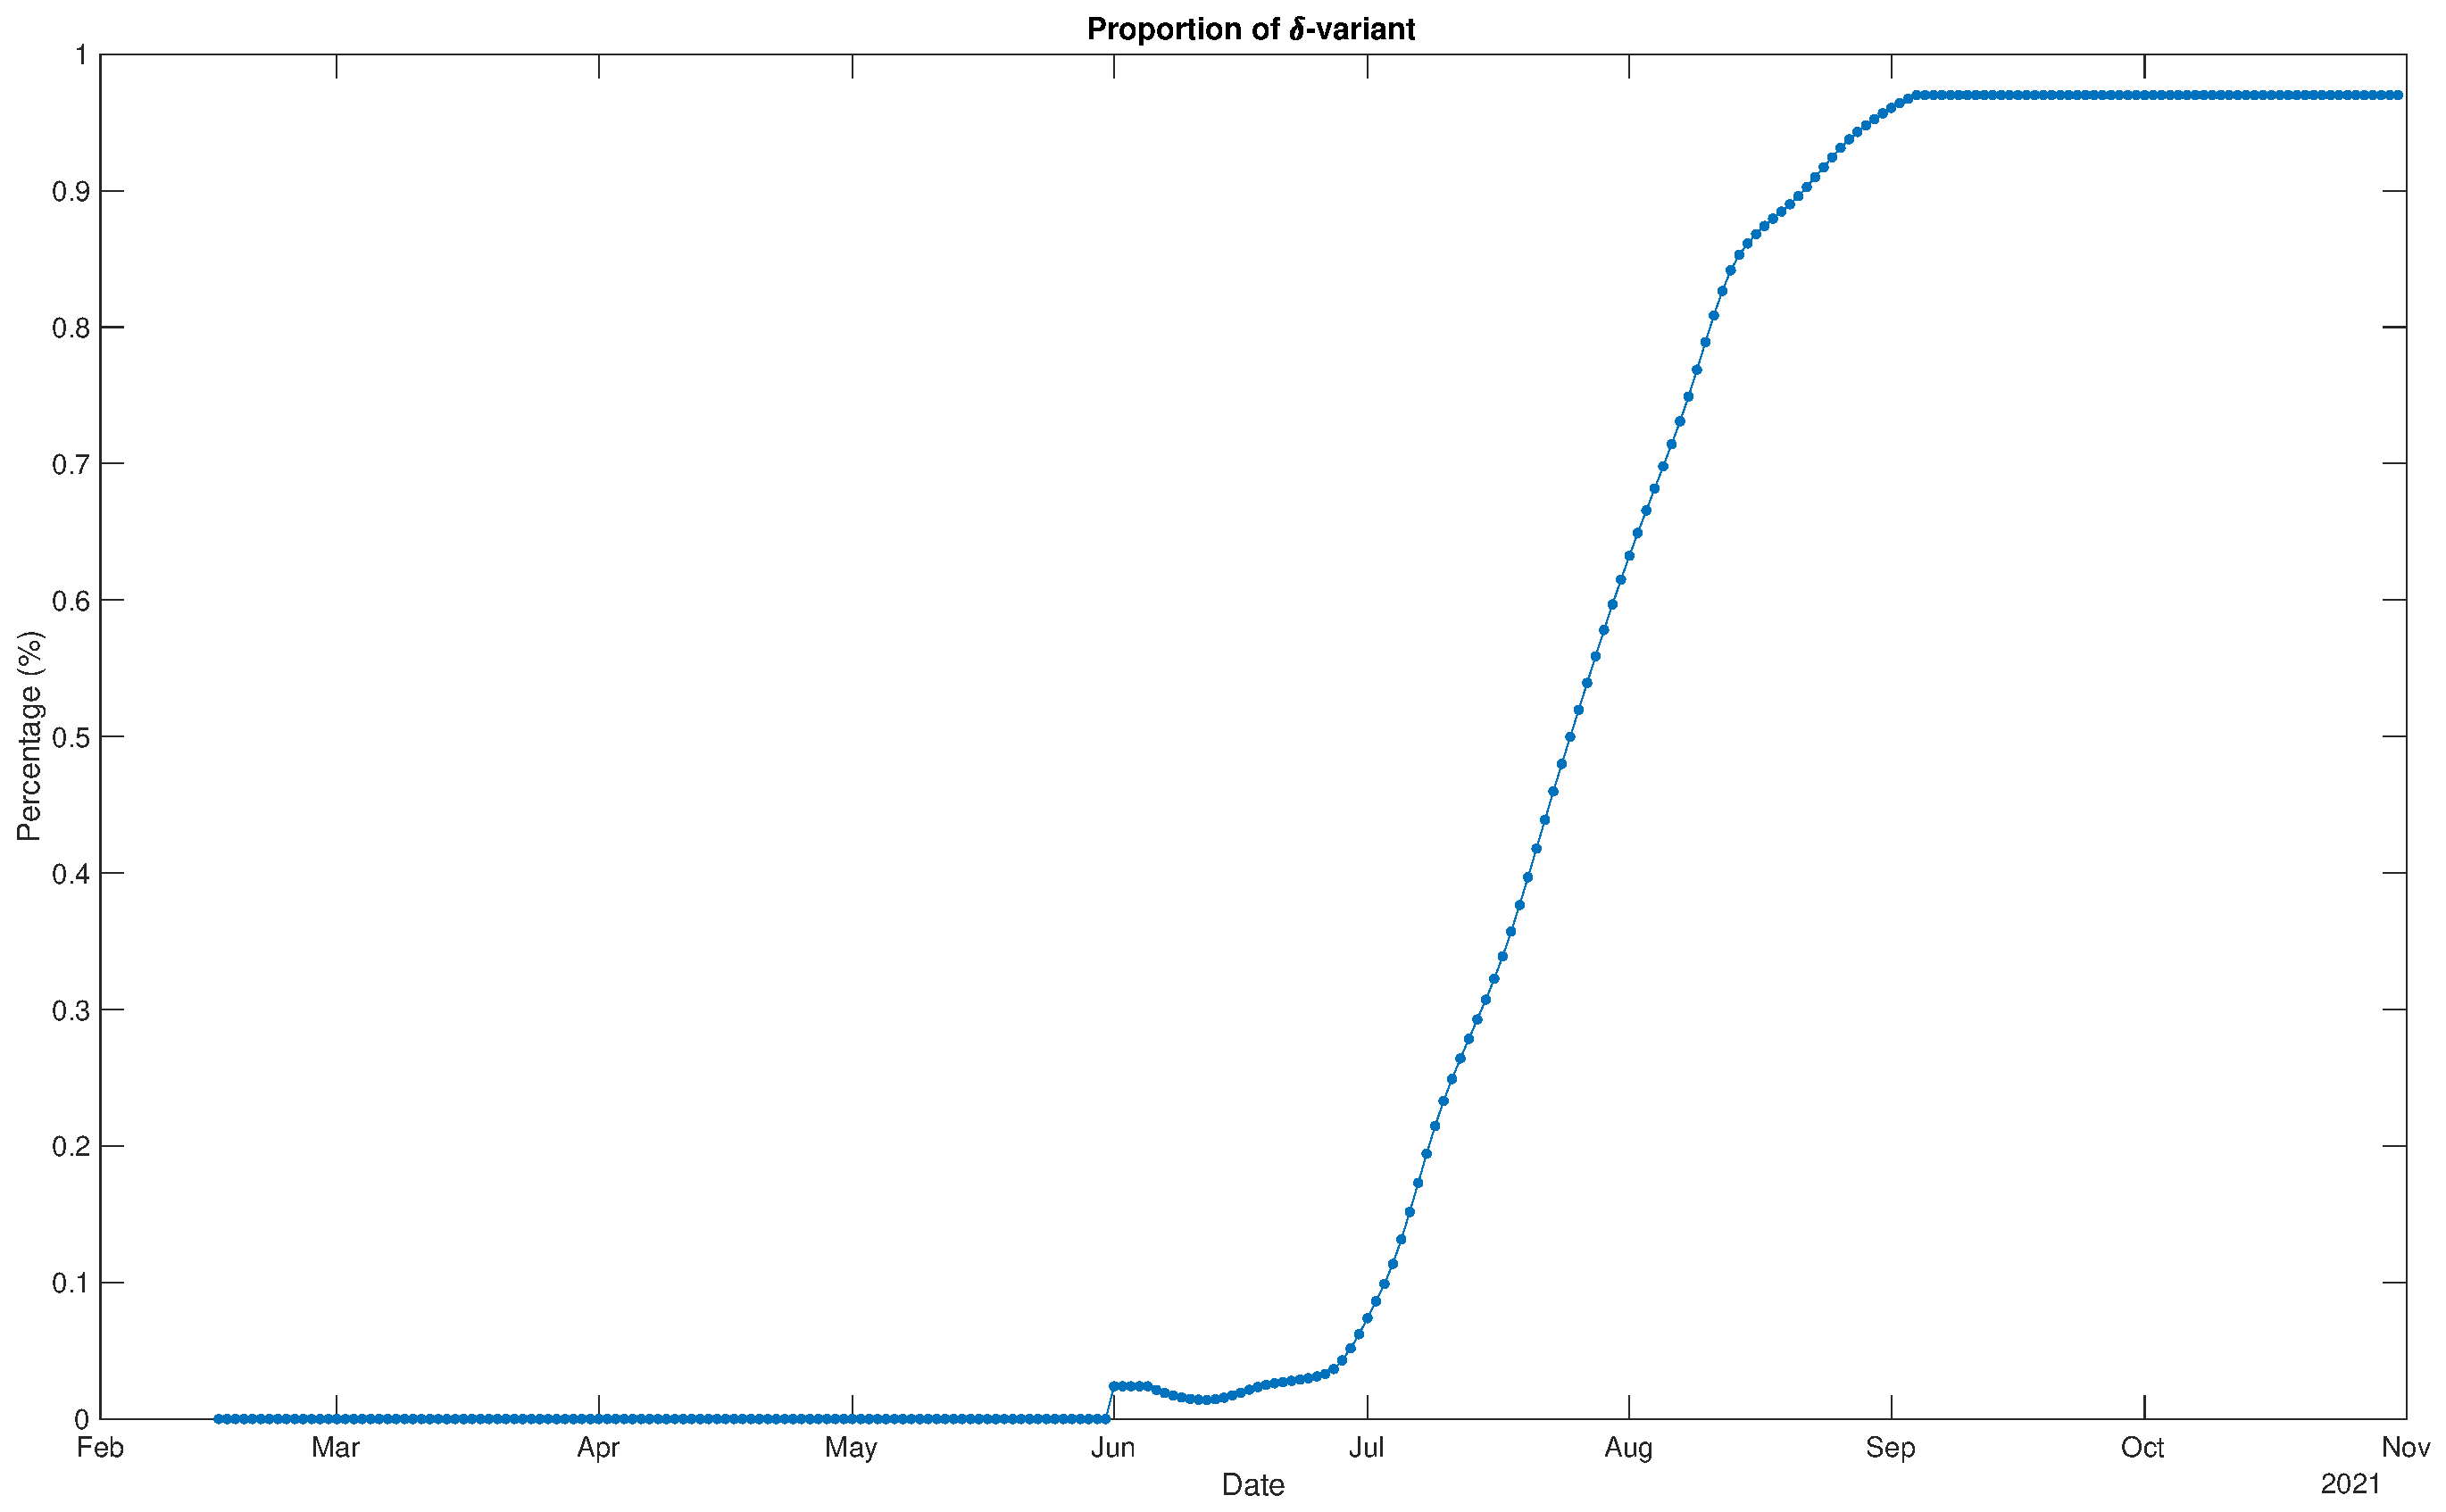
\includegraphics[width=\textwidth]{../results/data/delta_proportion.eps}
	    		\caption{추정한 $\delta$ 변이 비율}
	    	\end{figure}
	    \end{minipage}
	\end{frame}

	\begin{frame}\frametitle{데이터}
	    \textbf{백신 효과}
		\begin{itemize}
			\item $\delta$ 변이의 비율을 보도자료로부터 추정하고 weighted sum을 이용하여 백신 효과를 추정.
		\end{itemize}
		\begin{figure}
			\centering
			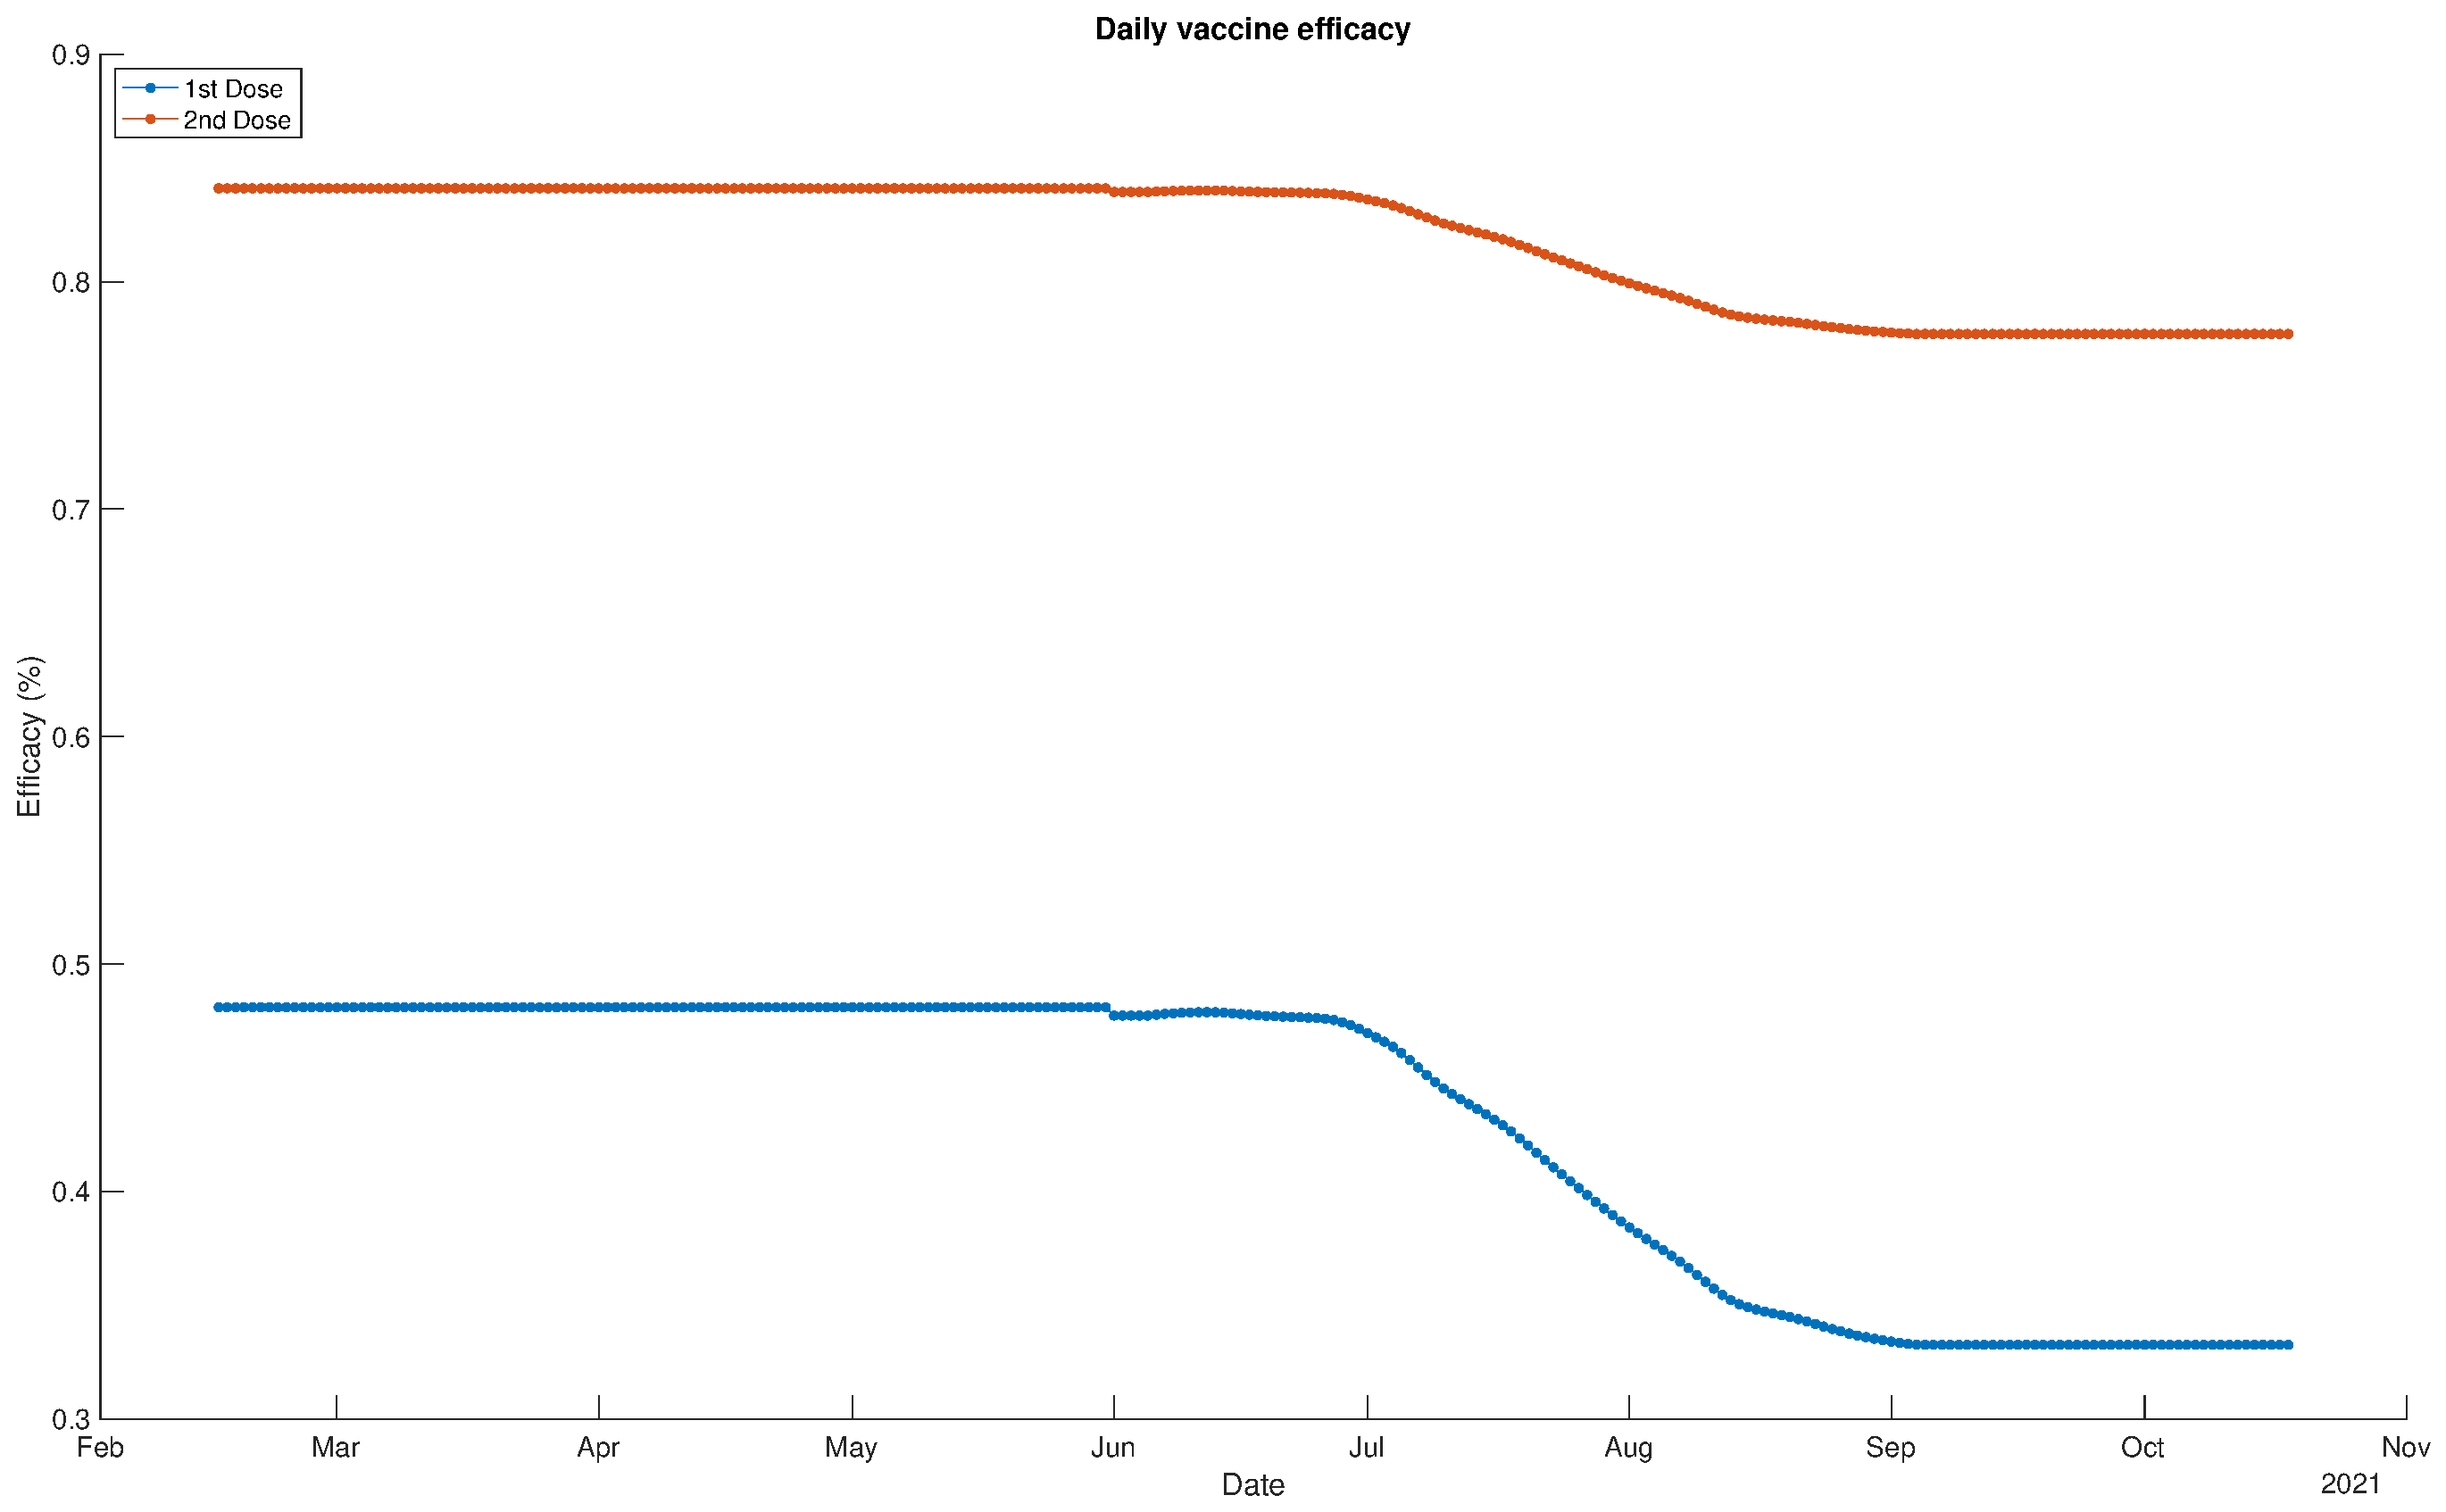
\includegraphics[width=9cm]{../results/data/vaccine_efficacy.eps}
			\caption{추정된 1차, 2차 백신의 일일 효과.}
		\end{figure}
	\end{frame}

	\begin{frame}\frametitle{데이터}
		\textbf{백신 효과}
	    \begin{table}
	    	\begin{tabular}{cr}
	    		\toprule
	    		 & \textbf{백신 위중증 예방 효과} \\
	    		\midrule
	    		\textbf{1차} & 75\%\footnotemark[2] \\
	    		\textbf{2차} & 94\%\footnotemark[2] \\
	    		\bottomrule
	    	\end{tabular}
	    	\hspace{1cm}
	    	\begin{tabular}{cr}
	    		\toprule
	    		 & \textbf{백신의 사망 예방 효과} \\
	    		\midrule
	    		\textbf{1차} & 85\%\footnotemark[3] \\
	    		\textbf{2차} & 96.1\%\footnotemark[4] \\
	    		\bottomrule
	    	\end{tabular}
	    	\caption{백신 차수별 위중증 (왼쪽) 및 사망 (오른쪽) 예방 효과}
	    \end{table}
	    \footnotetext[2]{\fullcite{stowe2021}}
	    \footnotetext[3]{\fullcite{bernal2021effectiveness}}
	    \footnotetext[4]{\fullcite{kdca2021}}
	\end{frame}

	\begin{frame}\frametitle{데이터}
		\textbf{사용 중인 위중증 병상 수}
	    \begin{figure}
	    	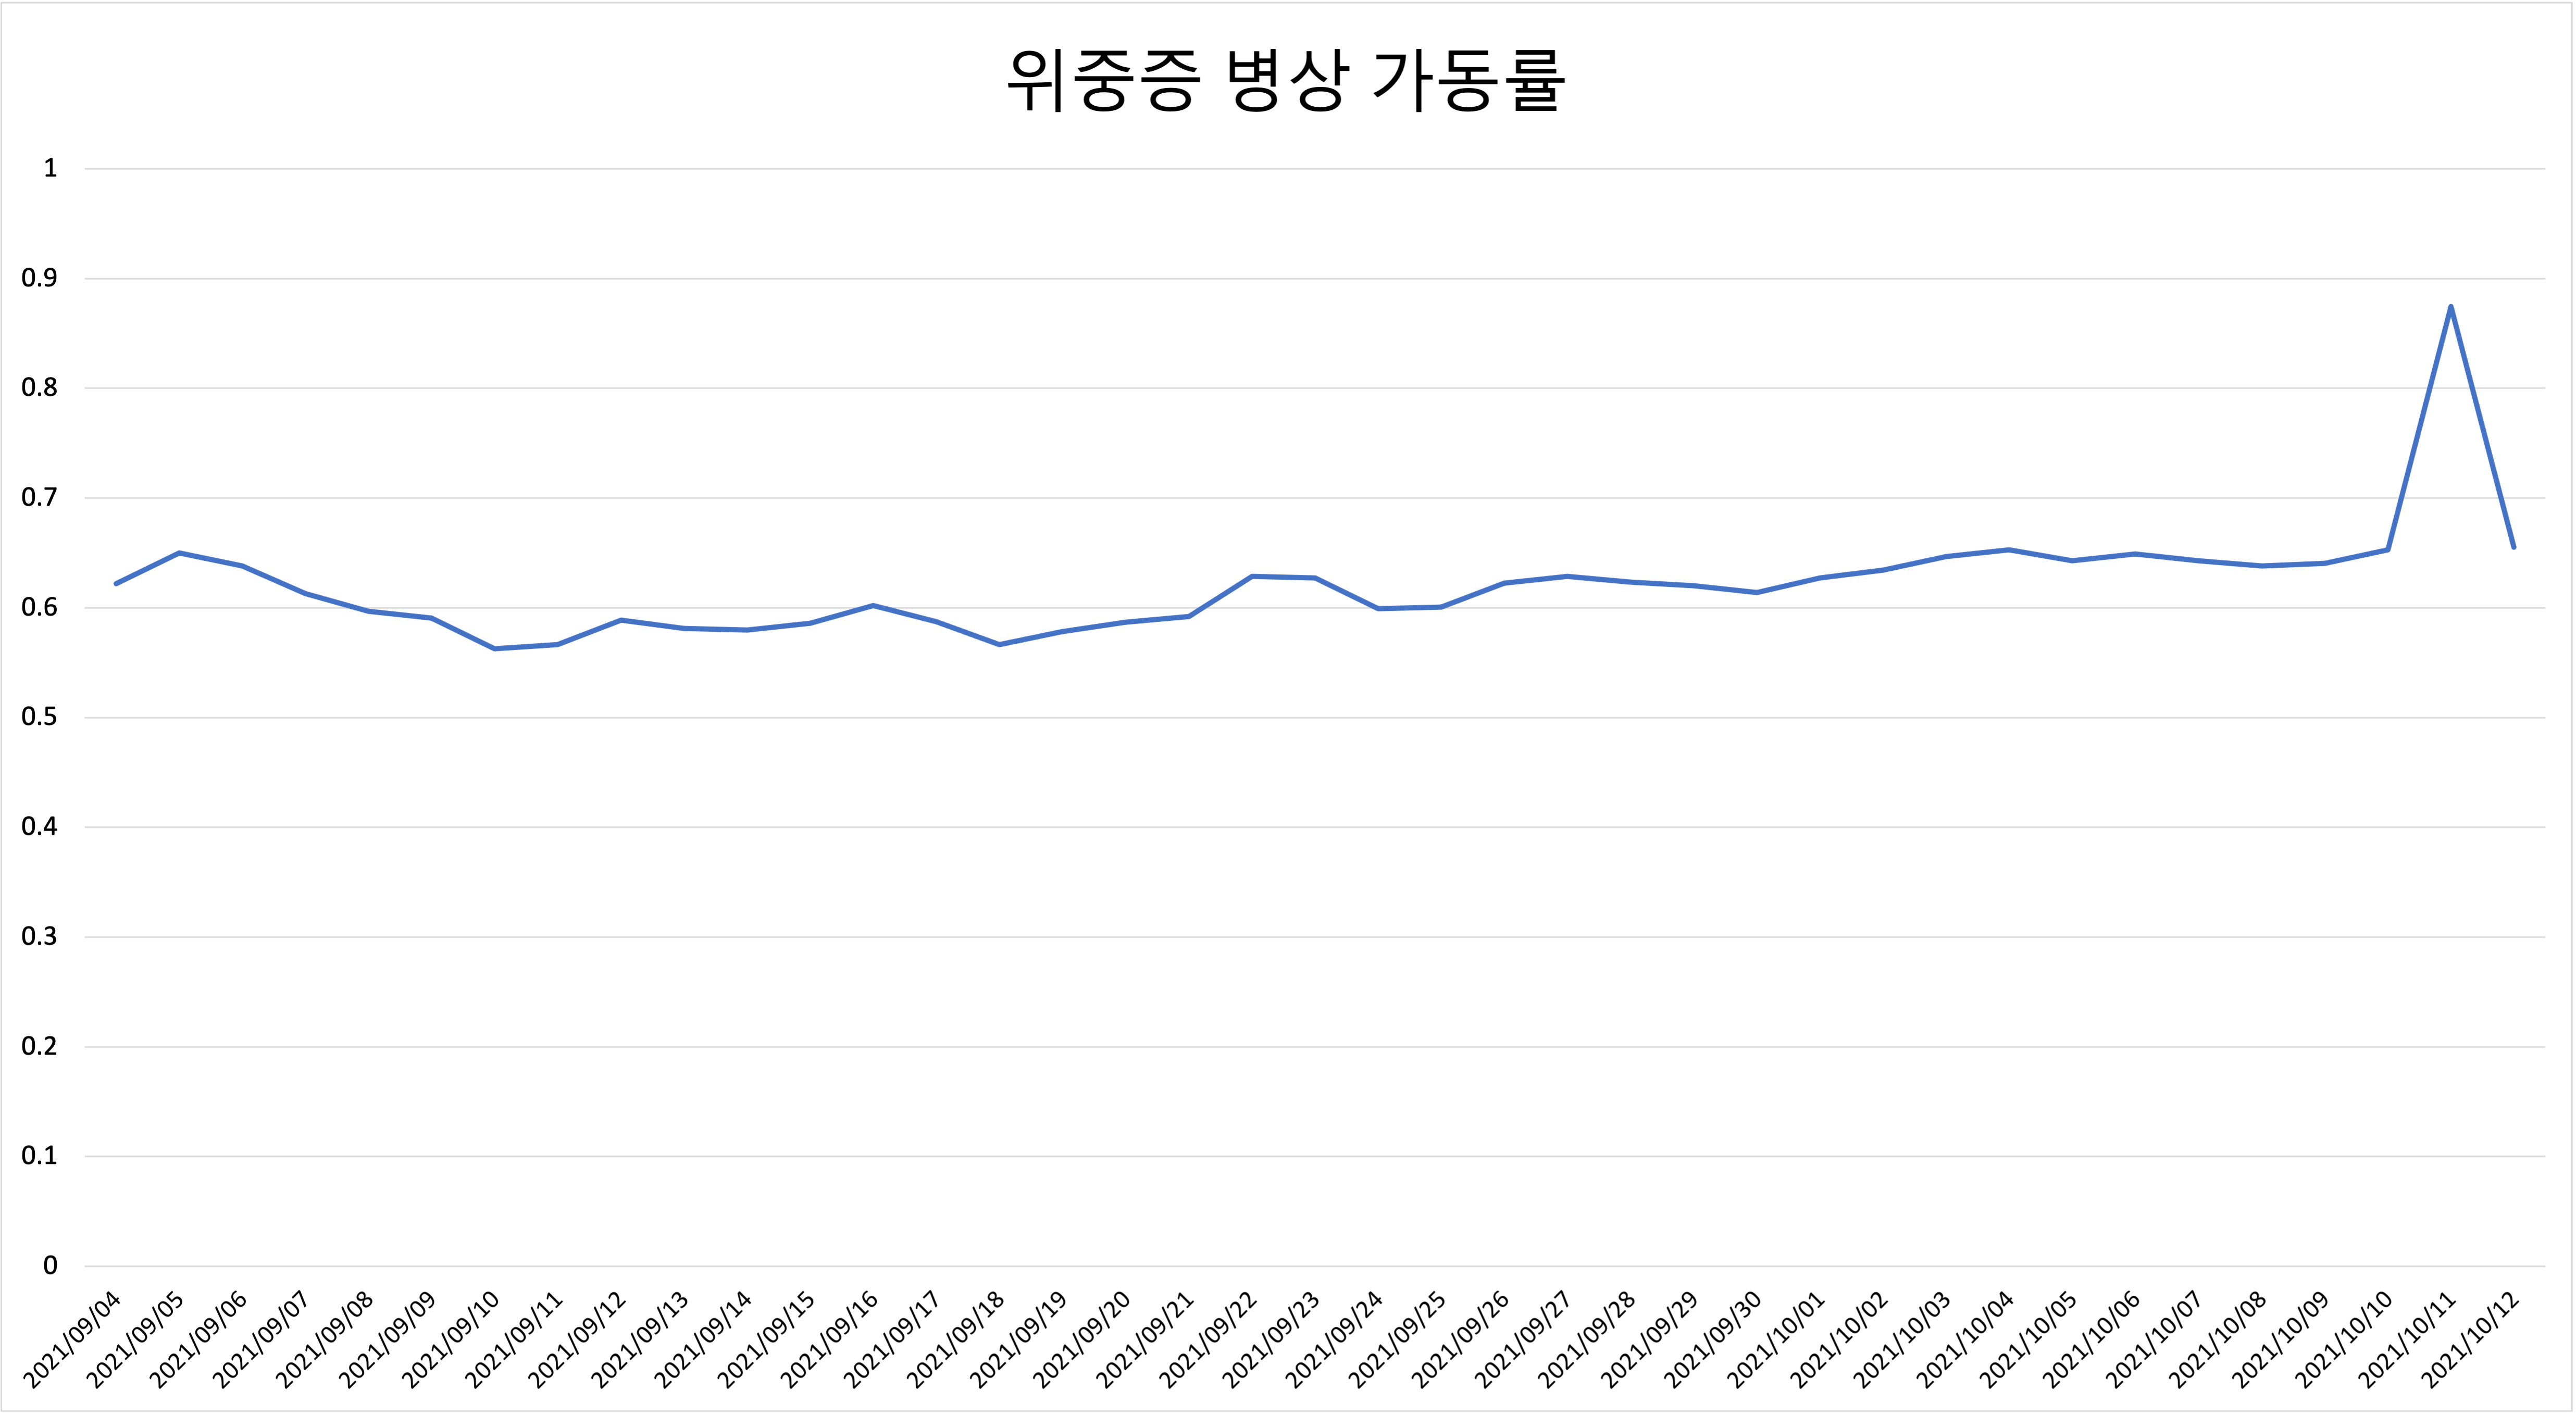
\includegraphics[width=10cm]{beds.png}
	    	\caption{사용 중인 위중증 병상 수}
	    \end{figure}
	\end{frame}

	\begin{frame}\frametitle{모델}
	    \begin{figure}
	    	\centering
	    	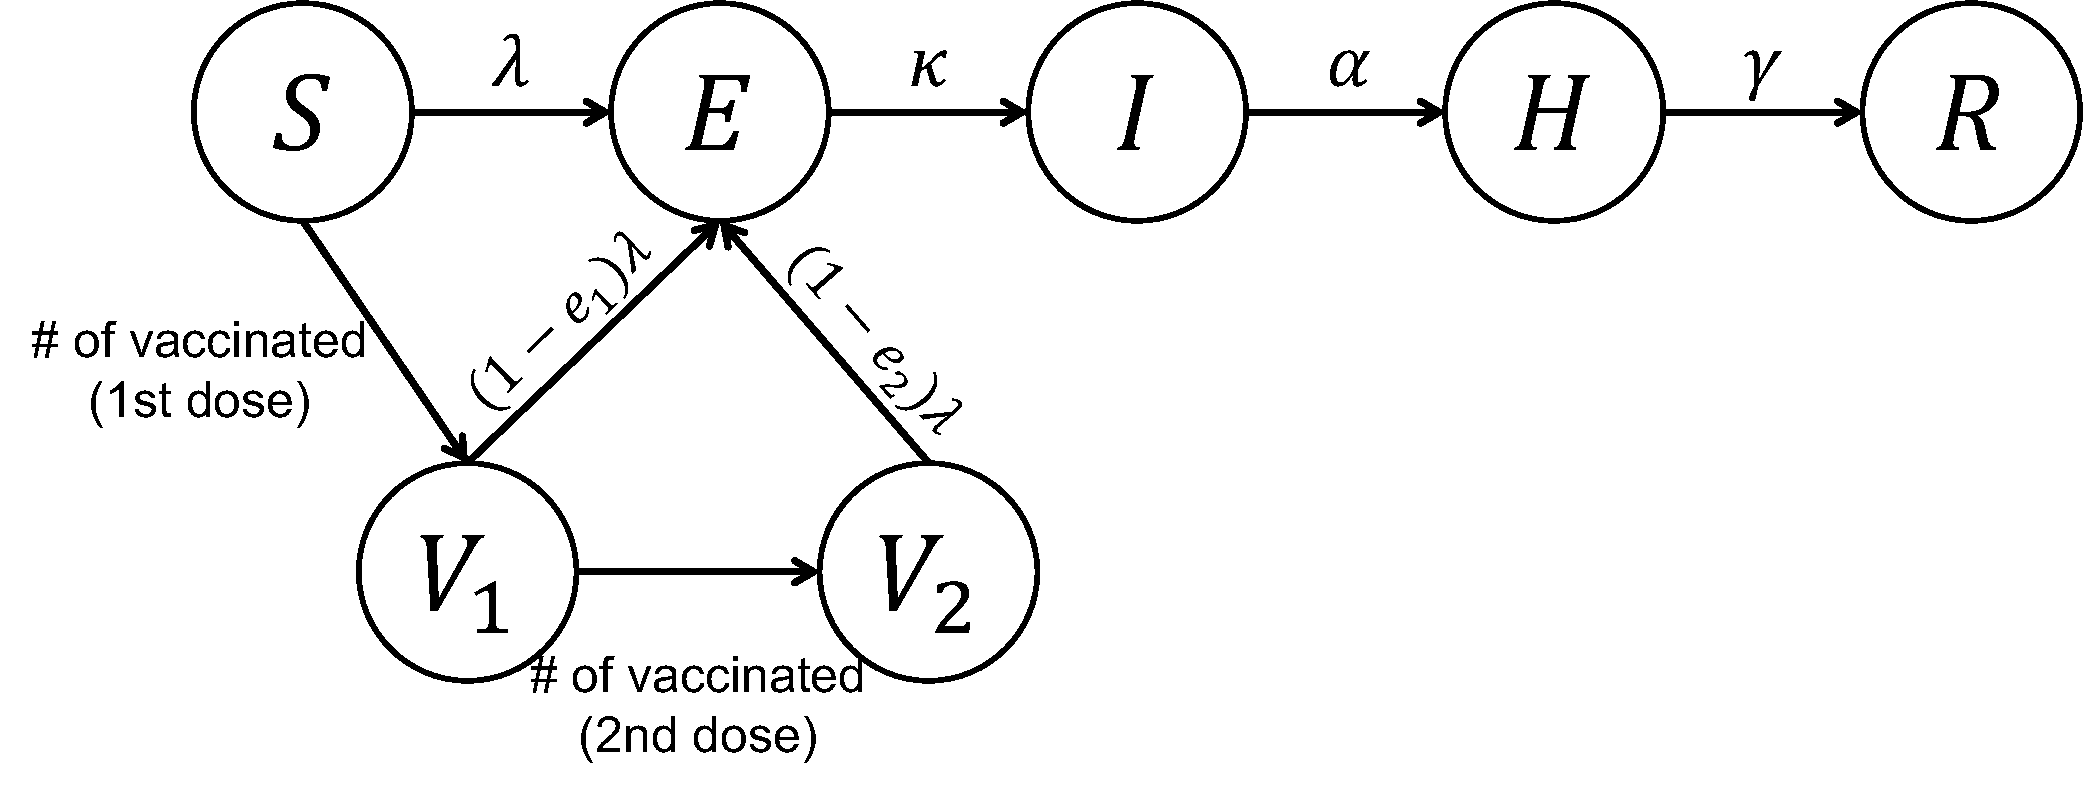
\includegraphics[width=12cm]{diagram.pdf}
	    	\caption{Diagram of age-structured model for SARS-CoV-2.}
	    \end{figure}
	\end{frame}

	\begin{frame}\frametitle{모델}
	    \begin{table}
	    	\begin{tabular}{cr}
	    		\toprule
	    		\textbf{Notation} & \textbf{Interpretation} \\
	    		\midrule
	    		$S$ & Susceptibles \\
	    		$E$ & Exposed \\
	    		$I$ & Infectious \\
	    		$H$ & Hospitalized \\
	    		$R$ & Removed (or recovered) \\
	    		$V_1$ & Vaccinated (1st dose) \\
	    		$V_2$ & Vaccinated (2nd dose) \\
	    		$\lambda$ & Force of infection \\
	    		$\kappa$ & Latent period \\
	    		$\alpha$ & Infectious period \\
	    		$\gamma$ & Hospitalization period \\
	    		$e_1$ & Vaccine efficacy for 1st dose \\
	    		$e_2$ & Vaccine efficacy for 2nd dose \\
	    		\bottomrule
	    	\end{tabular}
	    	\caption{Definition of states and parameters.}
	    \end{table}
	\end{frame}

	\begin{frame}\frametitle{모델 가정}
		\textbf{사회적 거리두기}
		\begin{itemize}
			\item 1단계 (구 0.5단계) 감소: transmission rate 전단계 대비 40\% 증가
			\item 1단계 (구 0.5단계) 증가: transmission rate 전단계 대비 32\% 감소
		\end{itemize}
	    \begin{table}
	    	\begin{tabular}{ccll}
	    		\toprule
	    		 & \textbf{날짜} & \textbf{사회적 거리두기 단계} & \textbf{transmission rate 변화} \\
	    		\midrule
	    		\multirow{2}{*}{고정} & 2021/02/15-2021/06/30 & 현 2단계 (구 2단계) &  \\
	    		 & 2021/07/01-2021/07/11 & 현 1단계 (구 1.5단계) & $\beta \times 1.4$ \\
	    		\midrule
	    		\multirow{3}{*}{가정}& \multirow{3}{*}{2021/07/12-2021/10/31} & 현 2단계 (구 2단계) & $\beta \times 1.4 \times 0.68$ \\
	    		 &  & 현 3단계 (구 2.5단계) & $\beta \times 1.4 \times 0.68^2$ \\
	    		 &  & 현 4단계 (구 3단계) & $\beta \times 1.4 \times 0.68^3$ \\
	    		\bottomrule
	    	\end{tabular}
	    	\caption{2021/02/15-2021/10/31 간의 사회적 거리두기와 transmission rate 변화, 모델의 가정.}
	    \end{table}
	\end{frame}

	\begin{frame}\frametitle{시나리오}
		\textbf{사회적 거리두기 (11월 이후)}
	    \begin{itemize}
	    	\item 현 상태 유지
	    	\item 1단계 완화
	    	\item 2단계 완화
	    	\item 11/1부터 1단계 완화, 12/13부터 2단계 완화
	    \end{itemize}
	    \vspace{0.3cm}
	    \textbf{등교 수준}
	    \begin{itemize}
	    	\item 현 상태 유지
	    	\item 현 1단계 수준 완화
	    	\item 현 2단계 수준 완화
	    	\item 전면 등교 및 마스크 미착용
	    \end{itemize}
	    \vspace{0.3cm}
	    \textbf{관찰 기간}
	    \begin{itemize}
	    	\item 2021/02/15-2021/12/31
	    \end{itemize}
	\end{frame}

	\foreach \sd in {same, 1, 2} {
		\foreach \sch in {same, 1, 2, max} {
			\begin{frame}\frametitle{시나리오: 11월 이후 사회적 거리두기 완화 수준 \sd단계,\, 등교 완화 수준 \sch단계}
				\begin{table}
					\begin{tabular}{CDDD}
						\toprule
						& \multicolumn{3}{c}{\textbf{7/12-10/31 거리두기 단계 효과}} \\
						\cmidrule{2-4}
						& \textbf{2단계} & \textbf{3단계} & \textbf{4단계} \\
						\midrule
						발생 & \includegraphics[width=3.5cm]{../results/predict_exp_1_sd3_\sd_school_\sch/incident_confirmed_all_age.eps} & \includegraphics[width=3.5cm]{../results/predict_exp_2_sd3_\sd_school_\sch/incident_confirmed_all_age.eps} & \includegraphics[width=3.5cm]{../results/predict_exp_3_sd3_\sd_school_\sch/incident_confirmed_all_age.eps} \\
						누적 & \includegraphics[width=3.5cm]{../results/predict_exp_1_sd3_\sd_school_\sch/cumul_confirmed_all_age.eps} & \includegraphics[width=3.5cm]{../results/predict_exp_2_sd3_\sd_school_\sch/cumul_confirmed_all_age.eps} & \includegraphics[width=3.5cm]{../results/predict_exp_3_sd3_\sd_school_\sch/cumul_confirmed_all_age.eps} \\
						\bottomrule
					\end{tabular}
					\caption{모델 가정에 따른 일일 발생 확진자 수 및 누적 확진자 수}
				\end{table}
			\end{frame}

			\begin{frame}\frametitle{시나리오: 11월 이후 사회적 거리두기 완화 수준 \sd단계,\, 등교 완화 수준 \sch단계}
				\begin{table}
					\begin{tabular}{CDDD}
						\toprule
						& \multicolumn{3}{c}{\textbf{7/12-10/31 거리두기 단계 효과}} \\
						\cmidrule{2-4}
						& \textbf{2단계} & \textbf{3단계} & \textbf{4단계} \\
						\midrule
						위중증 & \includegraphics[width=3.5cm]{../results/predict_exp_1_sd3_\sd_school_\sch/cumul_severe_all_age.eps} & \includegraphics[width=3.5cm]{../results/predict_exp_2_sd3_\sd_school_\sch/cumul_severe_all_age.eps} & \includegraphics[width=3.5cm]{../results/predict_exp_3_sd3_\sd_school_\sch/cumul_severe_all_age.eps} \\
						병상 & \includegraphics[width=3.5cm]{../results/predict_exp_1_sd3_\sd_school_\sch/num_beds.eps} & \includegraphics[width=3.5cm]{../results/predict_exp_2_sd3_\sd_school_\sch/num_beds.eps} & \includegraphics[width=3.5cm]{../results/predict_exp_3_sd3_\sd_school_\sch/num_beds.eps} \\
						\bottomrule
					\end{tabular}
					\caption{모델 가정에 따른 일일 누적 위중증 환자 수 및 필요 병상 수}
				\end{table}
			\end{frame}
		}
	}

\foreach \sch in {same, 1, 2, max} {
	\begin{frame}\frametitle{시나리오: 11/1 1단계 완화 후 12/13 2단계 완화, 등교 완화 수준 \sch단계}
	    \begin{table}
			\begin{tabular}{CDDD}
				\toprule
				& \multicolumn{3}{c}{\textbf{7/12-10/31 거리두기 단계 효과}} \\
				\cmidrule{2-4}
				& \textbf{2단계} & \textbf{3단계} & \textbf{4단계} \\
				\midrule
				발생 & \includegraphics[width=3.5cm]{../results/predict_exp_1_sd_constant_school_\sch/incident_confirmed_all_age.eps} & \includegraphics[width=3.5cm]{../results/predict_exp_2_sd_constant_school_\sch/incident_confirmed_all_age.eps} & \includegraphics[width=3.5cm]{../results/predict_exp_3_sd_constant_school_\sch/incident_confirmed_all_age.eps} \\
				누적 & \includegraphics[width=3.5cm]{../results/predict_exp_1_sd_constant_school_\sch/cumul_confirmed_all_age.eps} & \includegraphics[width=3.5cm]{../results/predict_exp_2_sd_constant_school_\sch/cumul_confirmed_all_age.eps} & \includegraphics[width=3.5cm]{../results/predict_exp_3_sd_constant_school_\sch/cumul_confirmed_all_age.eps} \\
				\bottomrule
			\end{tabular}
			\caption{모델 가정에 따른 일일 발생 확진자 수 및 누적 확진자 수}
		\end{table}
	\end{frame}

	\begin{frame}\frametitle{시나리오: 11/1 1단계 완화 후 12/13 2단계 완화, 등교 완화 수준 \sch단계}
		\begin{table}
			\begin{tabular}{CDDD}
				\toprule
				& \multicolumn{3}{c}{\textbf{7/12-10/31 거리두기 단계 효과}} \\
				\cmidrule{2-4}
				& \textbf{2단계} & \textbf{3단계} & \textbf{4단계} \\
				\midrule
				위중증 & \includegraphics[width=3.5cm]{../results/predict_exp_1_sd_constant_school_\sch/cumul_severe_all_age.eps} & \includegraphics[width=3.5cm]{../results/predict_exp_2_sd_constant_school_\sch/cumul_severe_all_age.eps} & \includegraphics[width=3.5cm]{../results/predict_exp_3_sd_constant_school_\sch/cumul_severe_all_age.eps} \\
				병상 & \includegraphics[width=3.5cm]{../results/predict_exp_1_sd_constant_school_\sch/num_beds.eps} & \includegraphics[width=3.5cm]{../results/predict_exp_2_sd_constant_school_\sch/num_beds.eps} & \includegraphics[width=3.5cm]{../results/predict_exp_3_sd_constant_school_\sch/num_beds.eps} \\
				\bottomrule
			\end{tabular}
			\caption{모델 가정에 따른 일일 누적 위중증 환자 수 및 필요 병상 수}
		\end{table}
	\end{frame}
}
	
\end{document}